\chapter{Direct multi-bed dynamic reconstruction: Supplementary material}
\label{chap:AppendixC}

Supplementary graphs, used in the analysis of the evaluated IsotoPK studies of chapter~\ref{Chap3_3:IsotoPK}, are provided here. Additionally, an brief simulation study for the behaviour of the spectral analysis model in the liver and the effects from the dual-input function is included.s

\section*{Supplementary graphs}

\begin{figure} [h!]
\centering
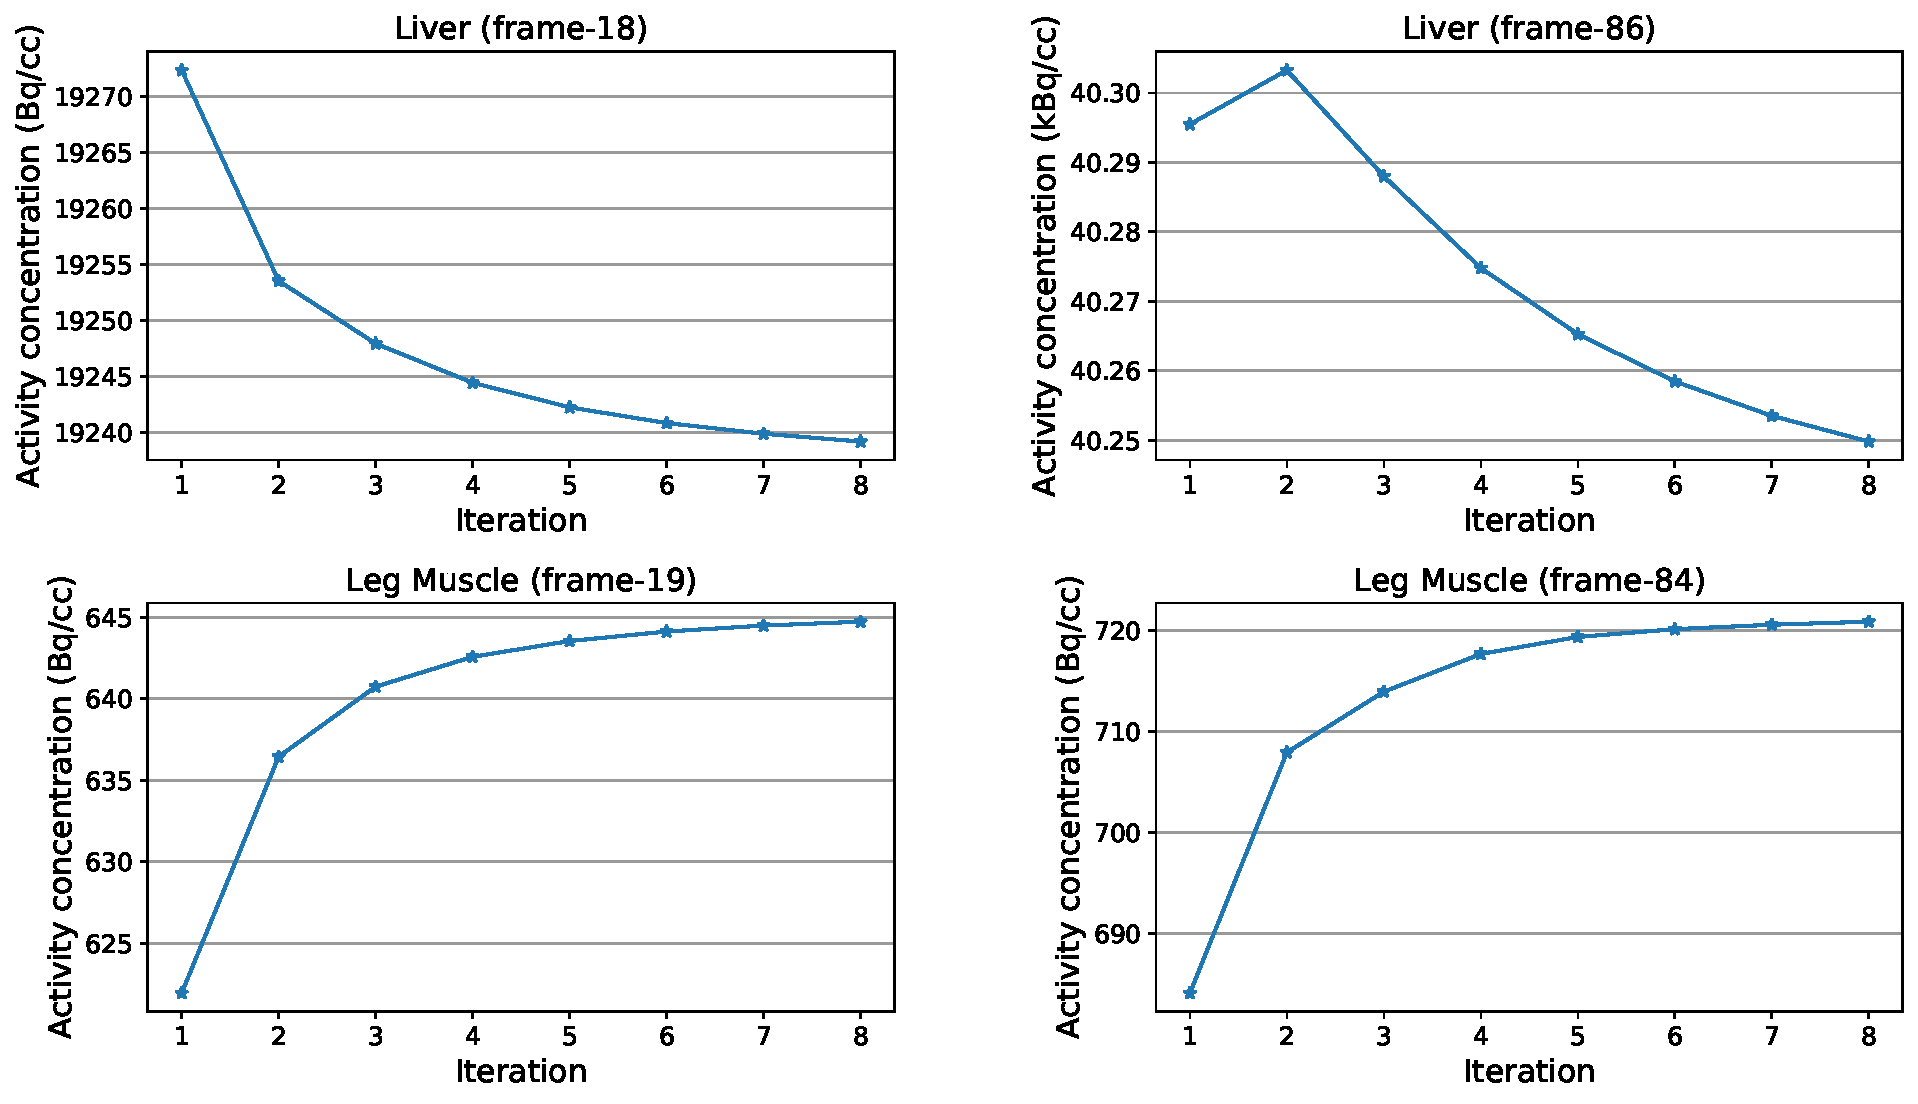
\includegraphics[scale=0.5,angle=0]{3_Results/3_3_DWB_Reconstruction/figures/3_3_IsotoPK_CTRL_DWB_3D_Convergence.pdf}
\caption{Liver (top) and Muscle (bottom) VOI mean versus iteration curves for 3D reconstruction. Shown for early (left) and late (right) frames of the \textit{CTRL} DWB acquisition including the DSB phase.}
\label{fig_3_3:IsotoPK_CTRL_DWB_4D_Convergence}
\end{figure} 

\begin{figure} [h!]
\centering
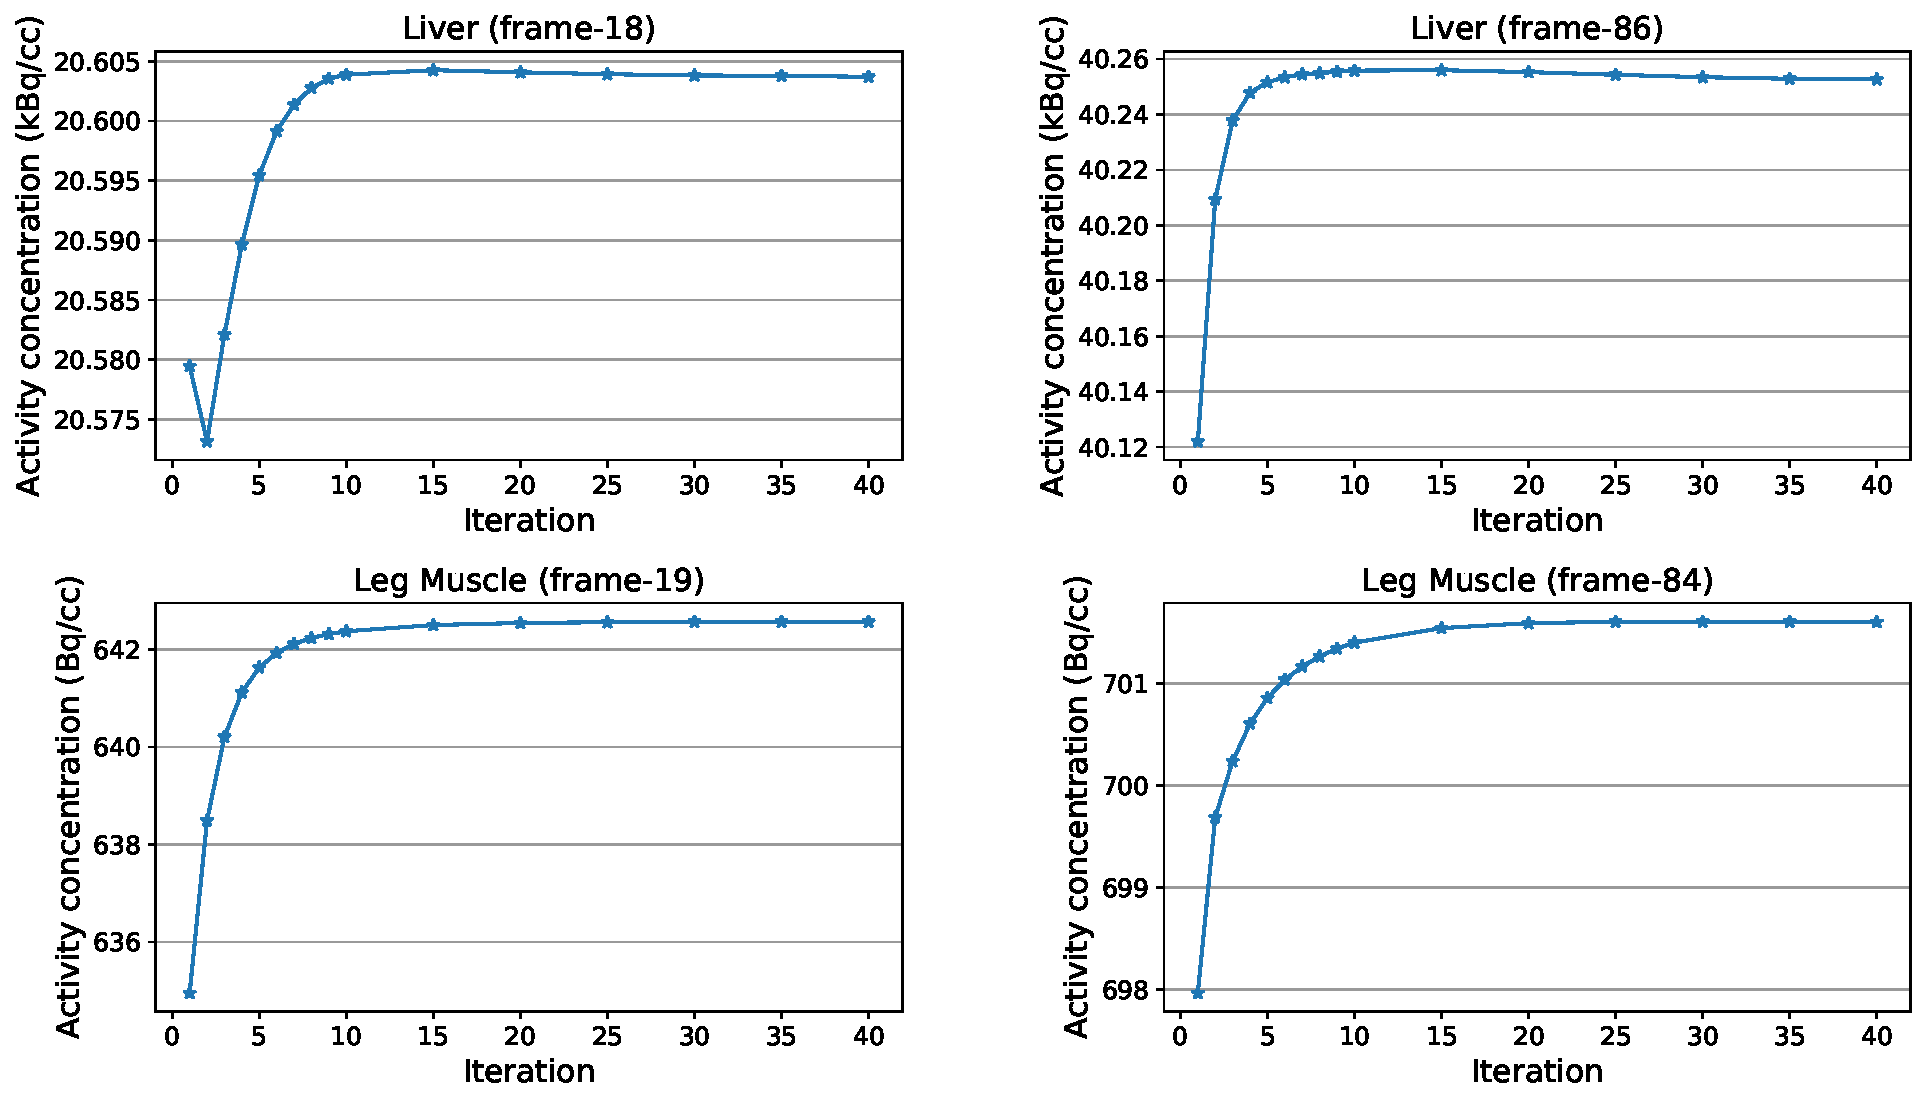
\includegraphics[scale=0.5,angle=0]{3_Results/3_3_DWB_Reconstruction/figures/3_3_IsotoPK_CTRL_DWB_4D_Convergence.pdf}
\caption{Liver (top) and Muscle (bottom) VOI mean versus iteration curves for 4D spectral reconstruction. Shown for early (left) and late (right) frames of the \textit{CTRL} DWB acquisition including the DSB phase.}
\label{fig_3_3:IsotoPK_CTRL_DSB_3D_Convergence}
\end{figure} 


\begin{figure} [h!]
\centering
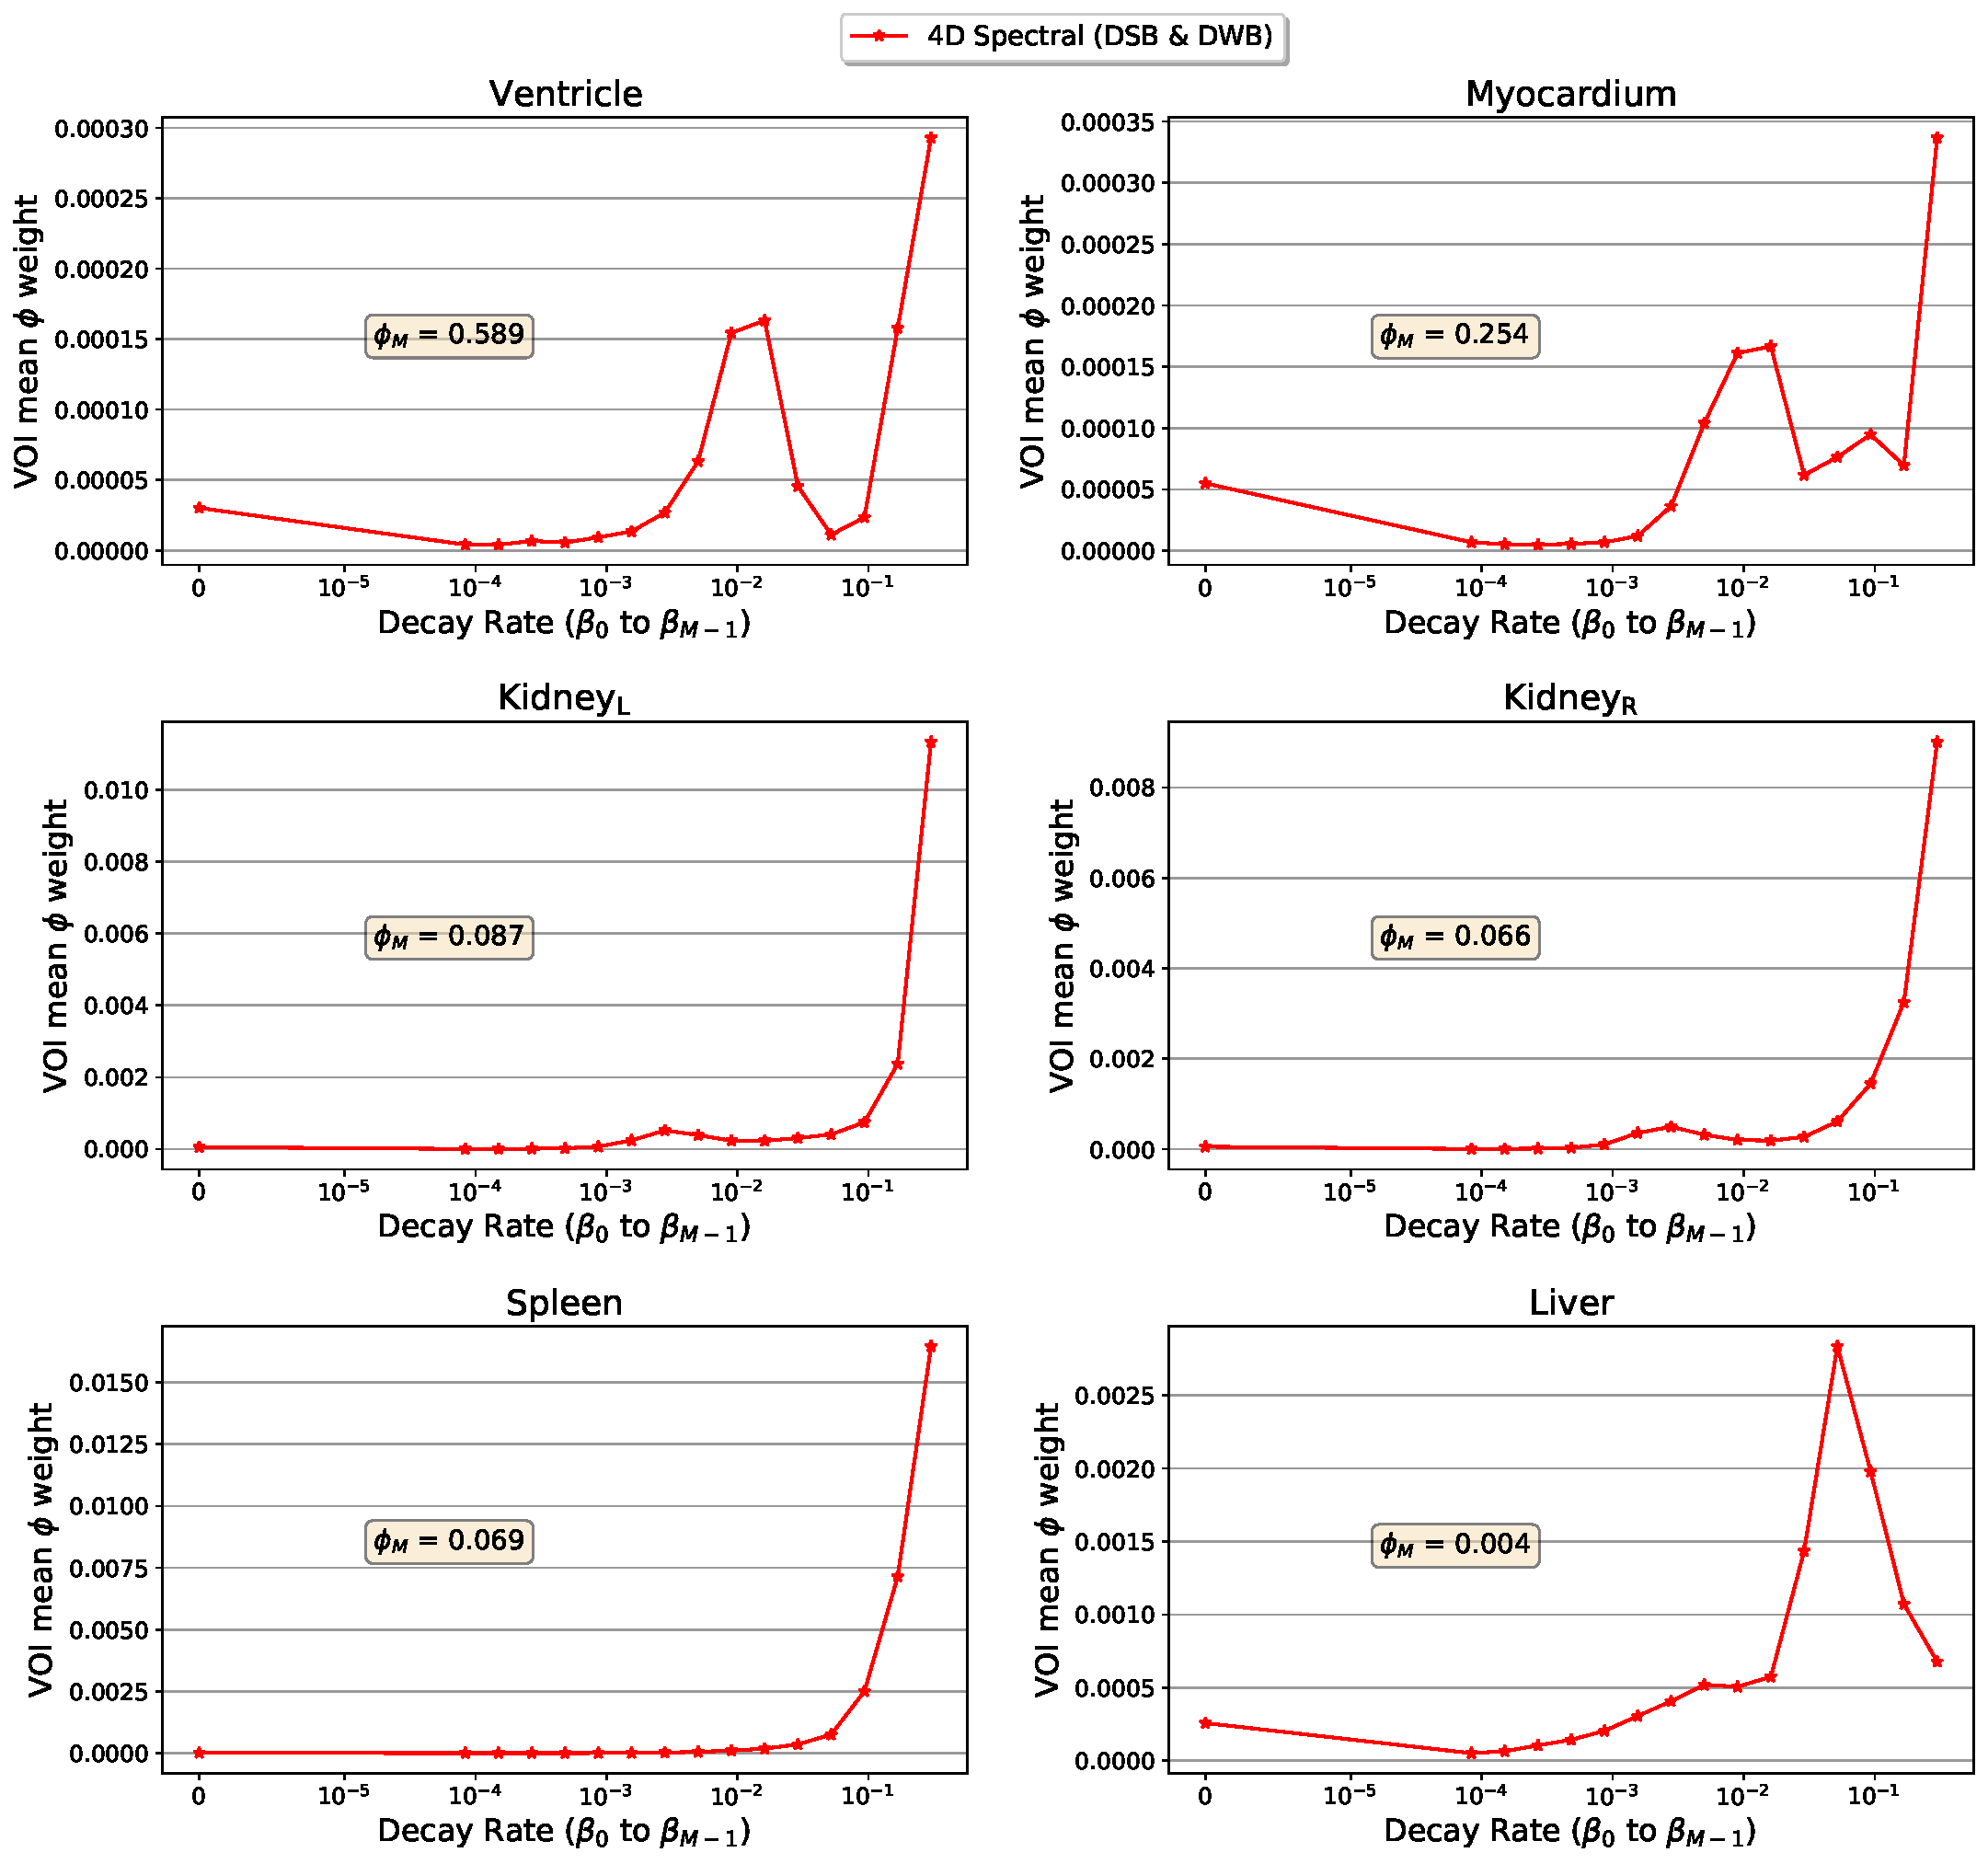
\includegraphics[scale=0.48,angle=0]{3_Results/3_3_DWB_Reconstruction/figures/3_3_IsotoPK_CTRL_DWB_SpectralParams_central_.pdf}
\caption{Spectral model coefficients average in VOIs. VOI regions shown which are included in both DSB and DWB acquisition.}
\label{fig_3_3:IsotoPK_CTRL_DWB_Spectrals}
\end{figure} 

\begin{figure} [h!]
\centering
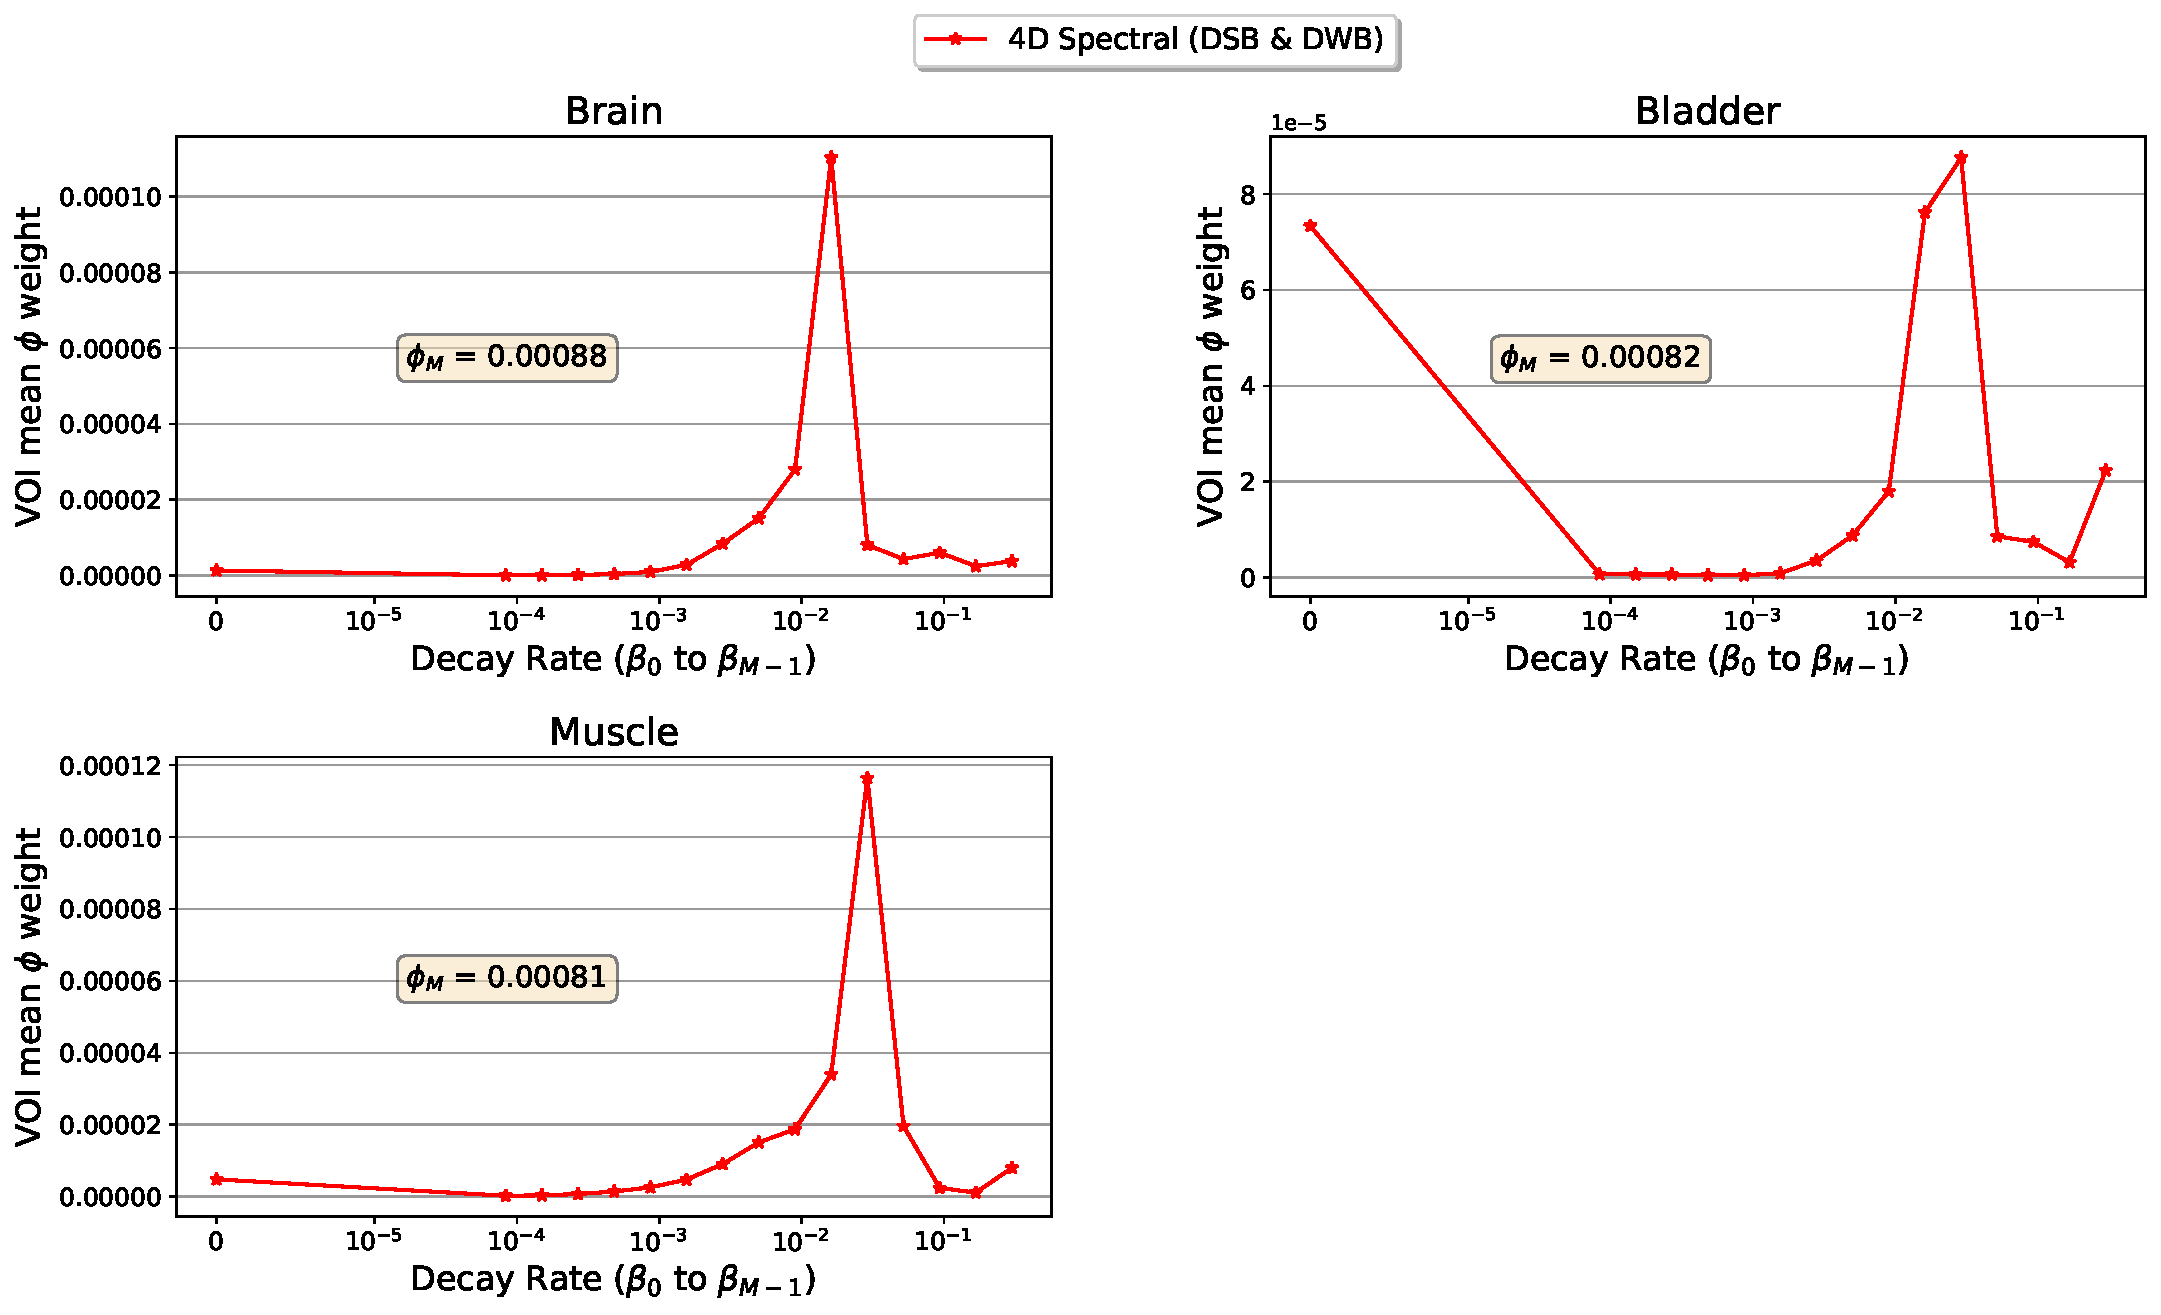
\includegraphics[scale=0.48,angle=0]{3_Results/3_3_DWB_Reconstruction/figures/3_3_IsotoPK_CTRL_DWB_SpectralParams_peripheral_.pdf}
\caption{Spectral model coefficients average in VOIs. VOI regions shown which are covered only by the DWB acquisition.}
\label{fig_3_3:IsotoPK_CTRL_DSB_Spectrals}
\end{figure} 

\clearpage
\section*{Liver dual-input sim study}
This short simulation was conducted using noiseless TACs to test the effects of the use of a dual input function model against spectral analysis that only accounts for one single input function.  
The following equations were used for the simulation. The portal vein input function was simulated using equation~\ref{eqn:Appendix_PortalVein} and a dispersion value $k_g=0.5 \mathrm{min}^{-1}$ from the literature~\cite{Kudomi2008}.
The dual input function was then simulated with a 25/75 ratio using equation~\ref{eqn:Appendix_HepaticInput} and provided to the equation~\ref{eqn:Appendix_2TCM} of the 2TC model for simulating liver TACs. Finally the blood fraction was included using equation~\ref{eqn:Appendix_CPET}. The simulated $K_1$ values varied between 0.3 and 2.4 min$^{-1}$. The simulated $k_2$, $k_3$ and $V_B$ values were 0.15 min$^{-1}$, 0.05 min$^{-1}$ and 0.03 respectively. These values, using a $K_1$= 0.7 min$^{-1}$, approach the TAC of the IsotoPK CTRL scan from chapter~\ref{Chap3_3:IsotoPK}. 
Spectral analysis was performed using the single input function of $C_{P}(t)$. 
%
\begin{equation} 
{C_{PV}}(t)  = {k_g} e^{-k_g t} \ast C_P(t)   \\ . \\
\label{eqn:Appendix_PortalVein}
\end{equation}
%
\begin{equation} 
{C_{H}}(t)  = 0.75 \cdot C_{PV}(t) + 0.25 \cdot C_{P}(t)  \\ . \\
\label{eqn:Appendix_HepaticInput}
\end{equation}
%
\begin{equation}
C_T(t) = K_1 ( e^{-(k_2+k_3)t} + \frac{k_3}{k_2+k_3}(1-e^{-(k_2+k_3)t})) \ast C_{H}(t)   
\label{eqn:Appendix_2TCM}
\end{equation}
%
\begin{equation}
{C_{PET}}(t)  = (1-V_{B}){C_{T}}(t) + V_{B}C_{H}(t) \\ , \\
\label{eqn:Appendix_CPET}
\end{equation}
%
%
The simulated TACs are shown in figure~\ref{fig_3_3:K1_Sims}, while the result $K_1^{*}$ values of the spectral analysis against simulated $K_1$ values are shown in~\ref{fig_3_3:K1_Sims_Results}. The results show an closely linear relationship between simulated $K_1$ and estimate $K_1^{*}$ values, with a deviation from a slope of 1. A part of this deviation is attributed to not correcting the $K_1^{*}$ values for blood fraction, but mostly it is due to unaccounted behaviour of the dual input function.
%
\begin{figure}[h!]
\centering
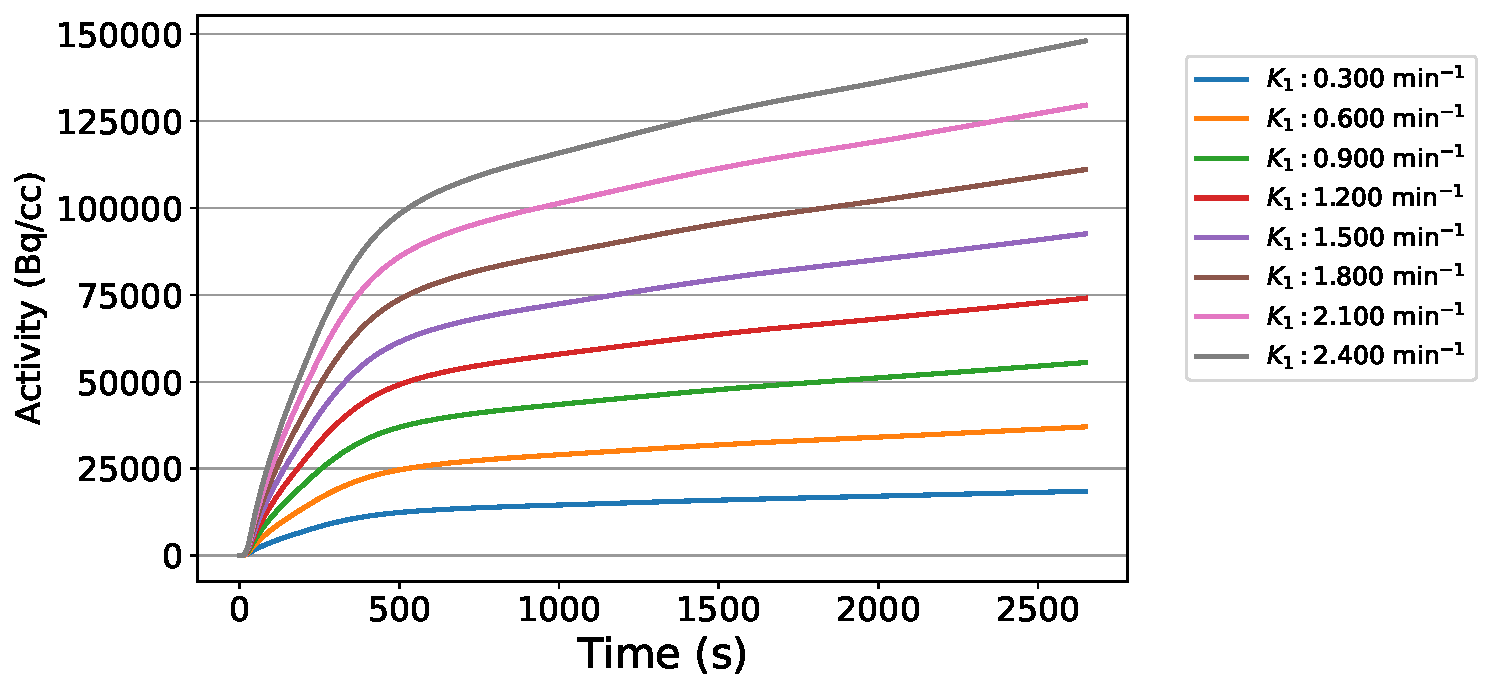
\includegraphics[scale=0.48,angle=0]{appendices/figures/ApendixC_multiple_K1.pdf}
\caption{Simulation of Liver TACs, using dual input function model and varying $K_1$ values}
\label{fig_3_3:K1_Sims}
\end{figure} 
%
\begin{figure}[h!]
\centering
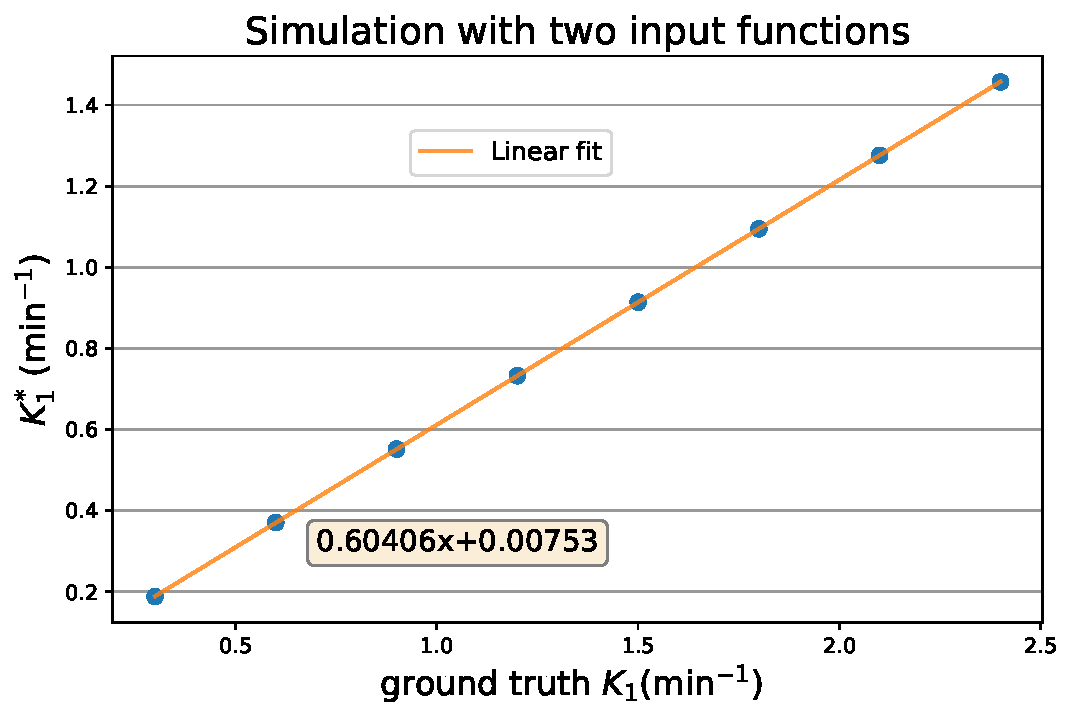
\includegraphics[scale=0.48,angle=0]{appendices/figures/ApendixC_multiple_K1_solution.pdf}
\caption{Simulation of Liver TACs, using dual input function model and varying $K_1$ values}
\label{fig_3_3:K1_Sims_Results}
\end{figure} 